\chapter{Lattice Models}
\label{sec:LM}
%
\noindent When we have a model for the free energy of a statistical mechanical system that is too complicated to
calculate analytically one approach is to utilize computers and \ac{mc} techniques. To make numerical
methods more effective one common approach is to discretize continuous models down on a 
numerical lattice. The lattice can in principle be of any form as long as the continuum limit reproduces
the original theory, however in this thesis we will exclusively focus on a square (cubic) numerical lattice
due to its simplicity.

In this chapter we will introduce different aspects of discretizing a continuous free-energy model down
on a square numerical lattice. If starting with a continuous model with a spatially dependent field
$f(\v{r})$, then the discretized model will have a corresponding field $f_\v{r}$ only defined on the
numerical lattice point sites at
\begin{equation}
    \label{eq:LM:latticeSites}
    \v{r} = \sum_\mu r_\mu\hat{\mu} = \sum_\mu a_\mu n_\mu\hat{\mu}
\end{equation}
where $a_\mu$ is the distance between lattice sites, $n_\mu\in[0,1,\ldots,N_\mu-1]$ and $N_\mu$ is the total number of sites in the $\mu$-direction.
The length of the numerical lattice in this direction is $L_\mu = a_\mu N_\mu$. The cubic numerical lattice
is specified by $a_\mu = a\;\forall\mu$ and $\mu\in\{x,y,z\}$.
Any integrals $\int\!\mathrm{d}^3r\;F[f(\v{r})]$ will
in such discretization have to be replaced with sums such that
\begin{equation}
    \label{eq:LM:integrals}
    \int\!\mathrm{d}^3r \mapsto a^3\sum_{r_\mu=a}^{Na}.
\end{equation}
If we are interested in bulk properties of the model in the thermodynamic limit, then specifying realistic
boundary conditions of the numerical lattice are of less importance. In this case, periodic boundary conditions
are from a computational perspective a convenient choice, which are defined by the requirement that
$f_{\v{r}+L_\mu\hat{\mu}} = f_\v{r}$ for any direction $\hat{\mu}$.

\section{Discretizing derivatives}

In a model where fields only are defined at discrete points in space, any spatial gradient of the fields must take the form
of discrete differences of the field values at these points. In a cubic grid of points with defined field-values such
differences can be denoted by the forward difference operator $\Delta_\mu$, which acts on a spatially discrete function $f_\v{r}$
as a forward difference in the direction of $\hat{\mu}$ such that
\begin{equation}
    \label{eq:LM:Derivatives:forwardDifference}
    \Delta_\mu f_\v{r} = f_{\v{r}+a\hat{\mu}} - f_\v{r},
\end{equation}
where $a$ is the distance between lattice points.
In a Euclidean geometry, then the natural discretization of a derivative $\partial_\mu$ is $\partial_\mu \mapsto \Delta_\mu/a$, which
reproduces the continuum derivative in the limit $a\rightarrow0$ with a fixed grid-size.
Using an appropriate set of units, we in most cases can set $a=1$.

\subsection{Covariant derivatives}

When discretizing continuous gauge theories, some extra care has to be taken when discretizing a covariant
derivative. Because of the gauge field, the geometry is no longer naively Euclidean such that we have to
rotate a field by a gauge group element to compare the field value at two spatially separate points. Given
a $U(1)$ gauge symmetry with gauge field components $A_\mu(\v{r})$, the appropriate way of discretizing a covariant derivative
is the identification \cite{shimizu12}
\begin{equation}
    \label{eq:LM:Derivatives:covariantDiscreteMapping}
    D_\mu f(\v{r}) = \big[\partial_\mu + igA_\mu(\v{r})\big]f(\v{r}) \mapsto \frac{1}{a}\big(f_{\v{r}+a\hat{\mu}}U_{\v{r},\mu} - f_\v{r}\big).
\end{equation}
The value of $f$ at $\v{r}+a\hat{\mu}$ is parallel transported back to $\v{r}$ by the $U(1)$ group element \cite{Munster2000}
\begin{equation}
    \label{eq:LM:Derivatives:U1ParallelTransporter}
    U_{\v{r},\mu} = e^{igA_{\v{r},\mu}},
\end{equation}
where
$g$ is the coupling constant between $f$ and the gauge field $A$, and
\begin{equation}
    \label{eq:LM:Derivatives:linkVariable}
    A_{\v{r},\mu} \equiv \int_\v{r}^{\v{r}+a\hat{\mu}}\!\mathrm{d}\v{r}\cdot\v{A}(\v{r}),
\end{equation}
is a link-variable, linking $\v{r}$ to its nearest neighbors.

In the limit of $a\to0$ this identification reproduces the covariant derivative%
\footnote{To show this, we see from Eq.~\eqref{eq:LM:Derivatives:linkVariable} that $A_{\v{r},\mu}\to aA_\mu(\v{r})$, expand the exponential
in $U_{\v{r},\mu}$ to first order and insert on the right hand side of Eq.~\eqref{eq:LM:Derivatives:covariantDiscreteMapping}.}%
. Furthermore it produces terms that transform in an analogous way to the continuum version under gauge transformations such that gauge
invariant terms remain invariant after discretization. In the continuous fields, a gauge transformation is defined by
\begin{equation}
    \label{eq:LM:Derivatives:gaugeTransformation}
    \begin{split}
        f(\v{r})&\to f(\v{r})e^{i\phi(\v{r})},\\
        A_\mu(\v{r})&\to A_\mu(\v{r}) - \frac{1}{g}\partial_\mu\phi(\v{r}).
    \end{split}
\end{equation}
Then the covariant derivative transforms as $D_\mu f(\v{r})\to e^{i\phi(\v{r})}D_\mu f(\v{r})$ such that terms such as $|D_\mu f(\v{r})|^2$
are invariant under gauge-transformations. Inserting the gauge transformation into the discretized field $f_\v{r}$ and the definition of the
link variables $A_{\v{r},\mu}$ we see that these discretized fields transform as
\begin{equation}
    \label{eq:LM:Derivatives:discretizedGaugeTransformation}
    \begin{split}
        f_\v{r}&\to f_\v{r}\,e^{i\phi_\v{r}},\\
        A_{\v{r},\mu}&\to A_{\v{r},\mu} - \frac{1}{g}\Delta_\mu\phi_\v{r},
    \end{split}
\end{equation}
where the field $\phi_\v{r}$ is discretely defined on the same lattice points as $f_\v{r}$. Inserting this into the
discretization of the covariant derivative on the right hand side of Eq.~\eqref{eq:LM:Derivatives:covariantDiscreteMapping} we see that indeed
the right hand side transforms in the same way as the left, \ie by picking up an overall factor $e^{i\phi_{\v{r}}}$. This means that
the discretized version of terms such as $|D_\mu f(\v{r})|^2$, which were originally gauge-invariant, will remain invariant after discretization
under the transformation in Eq.~\eqref{eq:LM:Derivatives:discretizedGaugeTransformation}.

\subsection{Reduction of symmetry}

One word of caution in this connection is that the discretized gradient terms will not necessarily have all the same spatial symmetries
as the originating continuous terms because the bias of the forward direction in the forward difference and the cubic structure of the numerical
lattice will in general break such symmetries. The effects of the cubic symmetry of the numerical lattice can be thought of as caused by
implicit lattice potentials that increases in influence towards lower temperatures and higher field strengths when the model contains an external
field
% TODO: cite
. Such lattice potentials can \eg cause topological defects to have
preferred positions in discretizations of theories with translational symmetry\footnote{More on this in Section~\ref{sec:Vor}.}.
As an example, consider again the discretization of the term
$\int\!\mathrm{d}^3r\;|\v{D}f(\v{r})|^2$ with discretized scalar field $f_\v{r}=\rho_\v{r}e^{i\theta_\v{r}}$. The density term is rotationally
symmetric%
\footnote{By rotationally symmetric we mean that if we were to rotate the field configurations of $f(\v{r})$ and $\v{A}(\v{r})$ in any direction,
by any amount, the term would still yield the same value.}
 in $3$D, however the discretized version can be written
\begin{equation}
    \label{eq:LM:Derivatives:discretizedKineticTerm}
    2\sum_\v{r}\sum_\mu\rho_\v{r}^2[1-\cos(\Delta_\mu \theta_\v{r}+gA_{\v{r},\mu})].
\end{equation}
From this form we can see that the term is only symmetric by rotation of $90^\circ$ in the planes normal to the $x$, $y$ and $z$ directions.
The discretized term contains cubic distortions when rotating in directions in-between these, hence the $SO(3)$ rotational symmetry is broken
down to the octahedral point group $O$.

The forward bias of the forward difference discretization scheme can also lead to breaking of symmetries that both the continuous model and the
numerical lattice have in common when the scalar field consists of multiple components. Consider a density term of the form
\begin{equation}
    \label{eq:LM:Derivatives:ExampleMG}
    \Re\Big[D_x\eta_xD_y\eta_y\Big],
\end{equation}
where $\eta_x$ and $\eta_y$ are two scalar fields that transform as components of spin such that under a $90^\circ$ $\hat{z}$-rotation
(which is called a $C_4$ transformation), then
$D_x\to D_y$, $D_y\to -D_x$, $\eta_x\to \eta_y$ and $\eta_y\to -\eta_x$. Inserting this into the continuous density term in 
Eq.~\eqref{eq:LM:Derivatives:ExampleMG} we see that it remains precisely the same \ie invariant. Now consider the discretization of this term,
which reads
\begin{equation}
    \label{eq:LM:Derivatives:ExampleMG:Discrete}
    \begin{split}
        &\rho^x_{\v{r}+\hat{x}}\rho^y_{\v{r}+\hat{y}}\cos\big[\theta^x_{\v{r}+\hat{x}}-\theta^y_{\v{r}+\hat{y}}+g(A_{\v{r},x}-A_{\v{r},y})\big]\\
        - &\rho^x_{\v{r}+\hat{x}}\rho^y_\v{r}\cos(\theta^x_{\v{r}+\hat{x}} - \theta^y_\v{r} + gA_{\v{r},x})\\
        - &\rho^x_\v{r}\rho^y_{\v{r}+\hat{y}}\cos(\theta^x_\v{r}-\theta^y_{\v{r}+\hat{y}}-gA_{\v{r},y})\\
        + &\rho^x_\v{r}\rho^y_\v{r}\cos(\theta^x_\v{r}-\theta^y_\v{r}),
    \end{split}
\end{equation}
where we have used the notation $\eta^a_\v{r} = \rho^a_\v{r}e^{i\theta^a_\v{r}}$ for the discrete scalar fields. In terms of these scalar fields
and link variables, a $C_4$ transformation consists of the mappings $\eta^x_\v{r}\to\eta^y_{C_4\v{r}}$, $\eta^y_\v{r}\to-\eta^x_{C_4\v{r}}$
such that \eg $\rho^x_{\v{r}+\hat{x}} \to \rho^y_{\v{r}'+\hat{y}}$. The link-variables transform as $A_{\v{r},\mu}\to A_{C_4\v{r},C_4\mu}$ such
that \eg $A_{\v{r},y}\to A_{\v{r}',-x}=-A_{\v{r}'-\hat{x},x}$. Using these transformations, and shifting the summation index of the 
external $\v{r}$-sum, then the rotated discrete terms take the form
\begin{equation}
    \label{eq:LM:Derivatives:ExampleMG:Discrete:Rotated}
    \begin{split}
        -&\rho^x_{\v{r}-\hat{x}}\rho^y_{\v{r}+\hat{y}}\cos\big[\theta^x_{\v{r}-\hat{x}}-\theta^y_{\v{r}+\hat{y}}-g(A_{\v{r},y}+A_{\v{r}-\hat{x},x})\big]\\
        +&\rho^x_\v{r}\rho^y_{\v{r}+\hat{y}}\cos(\theta^x_\v{r} - \theta^y_{\v{r}+\hat{y}}-gA_{\v{r},y})\\
        +&\rho^x_{\v{r}-\hat{x}}\rho^y_\v{r}\cos(\theta^x_{\v{r}-\hat{x}}-\theta^y_\v{r}-gA_{\v{r}-\hat{x},x})\\
        -&\rho^x_\v{r}\rho^y_\v{r}\cos(\theta^x_\v{r}-\theta^y_\v{r}),
    \end{split}
\end{equation}
which certainly is not the same as Eq.~\eqref{eq:LM:Derivatives:ExampleMG:Discrete}, \ie the discretization of Eq.~\eqref{eq:LM:Derivatives:ExampleMG}
is not invariant under a $C_4$ rotation. A more immediate way of seeing the problem is to recognize that the first term in
Eq.~\eqref{eq:LM:Derivatives:ExampleMG:Discrete} is a next-nearest neighbor coupling on the numeric lattice that only couples sites along one diagonal,
but not the other as illustrated in Figure~\ref{fig:LM:Derivatives:nextNearestDiagonalCoupling}, thus rotational symmetry is broken by the discretization.

\newcommand\latticeSpacing{1.5}
\begin{figure}[h]
  \centering
  \begin{tikzpicture}[scale=1.0]
    \def\latticeSite[#1,#2]{% Defines a lattice site with illustrated couplings. Arguments are x,y positions and size
        \draw [violet, dashed, opacity=0.5] (#1+0.1,#2) -- (#1+\latticeSpacing-0.1,#2);
        \draw [violet, dashed, opacity=0.5] (#1,#2+0.1) -- (#1,#2+\latticeSpacing-0.1);
        \draw [green, opacity=0.5] (#1+\latticeSpacing-0.1,#2+0.1) -- (#1+0.1,#2+\latticeSpacing-0.1);
        \node [opacity=0.5] at (#1, #2) {\textbullet};
    }
    % Draw the regular lattice sites
    \foreach \x/\y in {0-\latticeSpacing/0, -\latticeSpacing/\latticeSpacing, 0/\latticeSpacing, \latticeSpacing/0, \latticeSpacing/-\latticeSpacing, 0/-\latticeSpacing, -\latticeSpacing/-\latticeSpacing}
        \latticeSite[\x,\y];
    % Draw the left border
    \foreach \y in {0, \latticeSpacing, -\latticeSpacing} {
        \draw [violet, dashed, opacity=0.5] (-\latticeSpacing-0.1,\y) -- (-\latticeSpacing-\latticeSpacing+0.1,\y);
        \draw [green, opacity=0.5] (-\latticeSpacing-0.1,\y+0.1) -- (-\latticeSpacing-\latticeSpacing+0.1,\y+\latticeSpacing-0.1);
    }
    % Draw the bottom border
    \foreach \x in {0, \latticeSpacing, -\latticeSpacing} {
        \draw [violet, dashed, opacity=0.5] (\x,-\latticeSpacing-0.1) -- (\x,-\latticeSpacing-\latticeSpacing+0.1);
        \draw [green, opacity=0.5] (\x+0.1,-\latticeSpacing-0.1) -- (\x+\latticeSpacing-0.1,-\latticeSpacing-\latticeSpacing+0.1);
    }
    % Draw midpoint
    \draw [violet, dashed, thick] (0.1,0) -- (\latticeSpacing-0.1,0);
    \draw [violet, dashed, thick] (0,0.1) -- (0,\latticeSpacing-0.1);
    \draw [green, thick] (\latticeSpacing-0.1,0.1) -- (0.1,\latticeSpacing-0.1);
    \node at (0, 0) {\textbullet};
    % Upper right point
    \draw [violet, dashed, opacity=0.5] (\latticeSpacing+0.1,\latticeSpacing) -- (\latticeSpacing+\latticeSpacing-0.1,\latticeSpacing);
    \draw [violet, dashed, opacity=0.5] (\latticeSpacing,\latticeSpacing+0.1) -- (\latticeSpacing, \latticeSpacing+\latticeSpacing-0.1);
    \node [opacity=0.5] at (\latticeSpacing,\latticeSpacing) {\textbullet};
    % Draw node text
    \foreach \nx/\ny/\n in {-1/1/$\scriptstyle\v{r}-\hat{x}+\hat{y}$, 0/1/$\scriptstyle\v{r}+\hat{y}$, 1/1/$\scriptstyle\v{r}+\hat{x}+\hat{y}$,%
    -1/0/$\scriptstyle\v{r}-\hat{x}$, 0/0/$\scriptstyle\v{r}$, 1/0/$\scriptstyle\v{r}+\hat{x}$, -1/-1/$\scriptstyle\v{r}-\hat{x}-\hat{y}$,%
    0/-1/$\scriptstyle\v{r}-\hat{y}$, 1/-1/$\scriptstyle\v{r}+\hat{x}-\hat{y}$}
    \node [right] at (\nx*\latticeSpacing,\ny*\latticeSpacing+0.2) {\n};
\end{tikzpicture}
\caption{Couplings between sites on a single $z$-layer of the numerical lattice from the discretization in Eq.~\eqref{eq:LM:Derivatives:ExampleMG:Discrete}
of the term $\Re\big[D_x\eta_xD_y\eta_y\big]$. On-site terms are illustrated by a point (\textbullet), while nearest neighbor and next-nearest neighbor couplings are
illustrated by dashed and solid lines respectively. The couplings obtained by evaluating Eq.~\eqref{eq:LM:Derivatives:ExampleMG:Discrete} at a point $\v{r}$ are
emphasized by being less transparent than the rest.}
  \label{fig:LM:Derivatives:nextNearestDiagonalCoupling}
\end{figure}

One remedy for this kind of problem is to re-establish the broken symmetry by an average over symmetry-transformed terms. In the case of the discretization of
$\Re\big[D_x\eta_xD_y\eta_y\big]$ in Eq.~\eqref{eq:LM:Derivatives:ExampleMG:Discrete}, the $C_4$ symmetry can thus be re-established by taking the average of 
Eq.~\eqref{eq:LM:Derivatives:ExampleMG:Discrete},
Eq.~\eqref{eq:LM:Derivatives:ExampleMG:Discrete:Rotated}, as well as the terms obtained by transforming the discretization in Eq.~\eqref{eq:LM:Derivatives:ExampleMG:Discrete}
by the rotations $C_4^2$ and $C_4^3$. Let $\mathcal{F}_\v{r}$ denote the density terms in Eq.~\eqref{eq:LM:Derivatives:ExampleMG:Discrete} and let $\mathcal{T}\mathcal{F}_\v{r}$
be the terms that result when transforming $\mathcal{F}$ by a symmetry transformation $\mathcal{T}$. The average of symmetry-transformed terms that re-establishes the $C_4$
rotational symmetry can then be written
\begin{equation}
    \label{eq:LM:Derivatives:ExampleMG:symmetrized}
    \begin{split}
        &\mathcal{F}_\v{r}^{\text{sym}} = \frac{1}{4}\sum_{\mathcal{T}\in\{\mathbb{1},C_4,C_4^2,C_4^3\}}\mathcal{T}\mathcal{F}_\v{r}\\
        &= \frac{1}{4}\sum_{hh'=\pm 1}hh'\rho^x_{\v{r}+h\hat{x}}\rho^y_{\v{r}+h'\hat{y}}\cos\big[\theta^x_{\v{r}+h\hat{x}}-\theta^y_{\v{r}+h'\hat{y}}+g(A_{\v{r},hx}-A_{\v{r},h'y})\big].
    \end{split}
\end{equation}
In this expression, the next-nearest neighbour couplings are along all diagonals around the point $\v{r}$ such that it is rotationally symmetric under $C_4$ and thus does not
explicitly break symmetries that both the original theory and the numerical lattice have in common. Such breaking of symmetries can, as we have shown above,
result from the naive application of a forward difference discretization scheme%
\footnote{The symmetric expression in Eq.~\eqref{eq:LM:Derivatives:ExampleMG:symmetrized} can be more easily obtained by the use of a different discretization procedure than
the discretization of the covariant derivative in Eq.~\eqref{eq:LM:Derivatives:covariantDiscreteMapping}. Taking the average of a forward and backward difference that
respects gauge-transformations we get the discretization mapping
\begin{equation*}
    D_\mu f(\v{r})\mapsto (e^{igA_{\v{r},\mu}}f_{\v{r}+\hat{\mu}}-e^{igA_{\v{r},-\mu}}f_{\v{r}-\hat{\mu}})/2.
\end{equation*}
Applying this symmetrized covariant discretization mapping to the density term in Eq.~\eqref{eq:LM:Derivatives:ExampleMG}, yields Eq.~\eqref{eq:LM:Derivatives:ExampleMG:symmetrized}.
} %
  when discretizing terms with multiple gradient-directions and components. In models with such terms, the symmetry averaged expression can then be useful in diminishing the effect of 
meta-stable states and faster convergence when investigating such models by means of numerical computation. Finally we would like to stress that both versions yield the same theory
in the continuum limit.

\section{Including an external field}
\label{sec:LM:Field}

The interaction between superconductors and magnetic fields is an essential aspect in the study of superconductors and thus we will need to be able to add external magnetic fields
to our models in order to study this interaction. An external field is usually thought of as a constant homogeneous magnetic field in a certain direction that is a parameter of
the problem rather than a variable. In other words we assume the magnetic flux to be the same everywhere and unchanging, and rather than ask what consequence the existance of a superconductor
has on this field, we are interested in the effects the field has on the superconducting state. Physically this situation is relevant \eg if a relatively small and thin sheet
of superconducting material is placed in between two strong electromagnets as illustrated in Figure~\ref{fig:LM:Field:externalField}.
\begin{figure}[t]
    \centering
    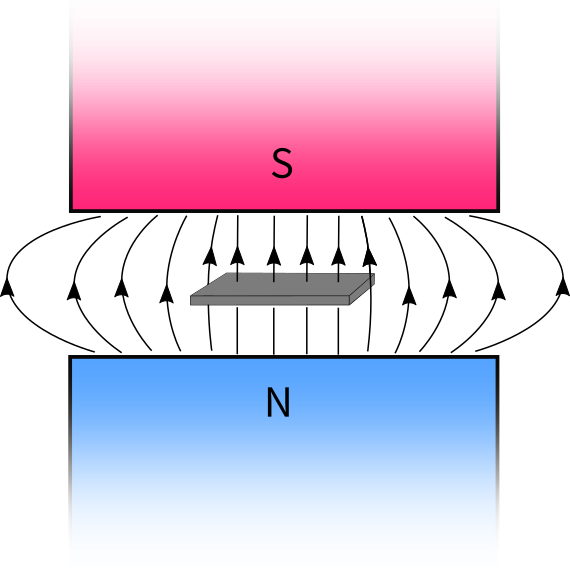
\includegraphics[width=0.45\textwidth]{external_field.png}
    \caption{A thin sheet of superconducting material in the magnetic field produced by two magnets pointing in the same direction above and below the superconductor.}
    \label{fig:LM:Field:externalField}
\end{figure}

One way to introduce a constant magnetic field in a lattice model is simply to figure out what kind of vector potential $\v{A}(\v{r})$ would give a constant magnetic field $\v{B}(\v{r})$
through $\v{B} = \nabla\times\v{A}$, and then set the link-variables $A_{\v{r},\mu}$ accordingly with the only caveat being that for a lattice-model with periodic boundary conditions,
then the factor $e^{igA_{\v{r},\mu}}$ has to satisfy periodic boundary conditions as well. This implies the condition
\begin{equation}
    \label{eq:LM:Field:periodicBC}
    \forall\nu\quad A_{\v{r},\mu} = A_{\v{r}+L_\nu\hat{\nu},\mu} + 2\pi m_\nu/g,
\end{equation}
where $m_\nu\in\mathbb{Z}$ and $\nu$ gives a direction on the lattice.

\subsection{Landau Gauge}
\label{sec:LM:Field:LandauGauge}

As an example, let's say we are interested in having an external field in the $\hat{z}$-direction with magnitude $B$. The vector-potential components $A_x$ and $A_y$ then have to satisfy
the equation
\begin{equation}
    \label{eq:LM:Field:vectorPotentialCondition}
    \partial_xA_y - \partial_yA_x = B.
\end{equation}
One configuration of the vector potential, which is called the \emph{Landau gauge}, that satisfies this condition is $A_y = Bx$ with the other vector potential components set to zero. Inserting
this into the definition of the link-variables in Eq.~\eqref{eq:LM:Derivatives:linkVariable} yields $A_{\v{r},\mu} = ar_xB\delta_{\mu,y}$. Here $x$ is a continuous variable while
$r_x$ is the $x$-component of a lattice vector. Periodic boundary conditions on the lattice implies the condition $A_{\v{r},y} = A_{\v{r}+L_x\hat{x},y} - 2\pi m/g$
which finally restricts the value of the field $B$ such that the link-variables in the Landau
gauge must take the form
\begin{equation}
    \label{eq:LM:Field:LandauGauge}
    A_{\v{r},\mu} = \delta_{\mu,y}r_x\frac{2\pi m}{gL_x},\quad m\in\mathbb{Z},
\end{equation}
where $L_x=N_xa$ and $N_x$ is the number of lattice sites in the $x$-direction. With this link-variable configuration, the field strength becomes $B = 2\pi f/ga^2$ where we have defined
the filling fraction $f=m/N_x$ which in terms of vortices gives the number of magnetic vortices pr. plaquette of the numerical lattice.

\subsection{Symmetric Landau gauge}
\label{sec:LM:Field:SymmLandauGauge}

The Landau gauge has the disadvantage that it singles out a direction in the $xy$-plane since the vector potential is set to $\v{A}(\v{r})=Bx\hat{y}$ and thus only spatially dependent
in the $x$-direction. It could because of this be argued to break a rotational symmetry of the model in the $xy$-plane given that Aharenov-Bohm-like effects are significant to the results.
To mitigate any such concern, one can consider a symmetric gauge given by the choice $\v{A}(\v{r}) = -\v{r}\times B\hat{z}/2$, which is rotationally symmetric in the $xy$-plane
and, like the Landau gauge, produces the field $\v{B} = B\hat{z}$.
Inserting this choice of vector potential into the link variables yields, using implicit summation over repeated indices,
$A_{\v{r},\mu} = \epsilon_{\mu z\nu}r_\nu aB/2$. Periodic boundary conditions in this case implies
two restrictions on the field value $B$ because the vector potential varies in both the $x$- and $y$-direction. Implementing these conditions we can write the link-variables as
\begin{equation}
    \label{eq:LM:Field:symmGaugeLinks}
    A_{\v{r},\mu} = \epsilon_{\mu z\nu}r_\nu\frac{2\pi m}{gL_x},
\end{equation}
where $m$ is a number $m\in\mathbb{Z}$ chosen such that there exists some $n\in\mathbb{Z}$ such that $mN_y=nN_x$, \ie $m$ is some multiple of $N_x/N_y$.
Then the field value is given by $B = 2\pi f/ga^2$ for filling fraction $f=2m/N_x$.

This gauge is a specification of the more general extended Landau gauge \cite{Nguyen99PRB,Nguyen99EPL}, which is borne purely out of the assumptions of a field $\v{B}\|\hat{z}$,
$\v{A}(\v{r})$ linear in $\v{r}$ and
periodic boundary conditions.

\subsection{Fluctuating field}

For a normal strongly type-II superconductor, the London penetration depth $\lambda$ is much larger than the superconducting coherence length $\xi$. In this regime it is valid to neglect
spatial fluctuations in the gauge field since any deviation around the extremal field configuration is strongly suppressed. This is called the frozen gauge approximation and
makes the vector potential act only as a constraint on the value of the uniform magnetic induction given by one of the gauges presented in the above sections \cite{Nguyen99PRB}.
When the superconducting state consists of multiple components on the other hand, it becomes difficult to classify it simply in terms of type-I or type-II based solely on
$\lambda$ and $\xi$ \cite{Babaev05}.
With multiple components, it becomes essential to fluctuate the gauge field, because it mediates a significant indirect interaction between the components \cite{Smorgrav05, Smiseth04}.

Fluctuations of the gauge field imparts an energy cost on the system given in SI-units by the free energy%
\footnote{One way of deriving said energy is to start with the sourceless
Maxwell Lagrangian for a massless vector field
$\mathcal{L}_M = -F^{\mu\nu}F_{\mu\nu}/4\mu_0$. In this relativistic notation $F^{\mu\nu} = \partial^\mu A^\nu-\partial^\nu A^\mu$, $A^0 = V$, $\partial_0 = \partial_t/c$ and we use  the
metric $g^{\mu\nu} = \diag(1, -1, -1, -1)$. Assuming time-independence and neglecting terms consisting only of $V$ since they do not couple to the Higgs fields (\eg the superconducting
components) in minimal coupling, then the Lagrangian reduces to $\mathcal{L}_M \to -(\nabla\times\v{A})^2/2\mu_0$ and the free energy in Eq.~\eqref{eq:LM:Field:Fluc:freeEnergy} results.}
\begin{equation}
    \label{eq:LM:Field:Fluc:freeEnergy}
    F_A = \frac{1}{2\mu_0}(\nabla\times\v{A})^2.
\end{equation}
There are a couple of different ways of discretizing this energy for inclusion in a lattice model depending on whether one defines the link-variables compactly,
\ie $gA_{\v{r},\mu} \in (-\pi, \pi)$, or non-compactly, \ie $gA_{\v{r},\mu} \in (-\infty,\infty)$. Both versions belong to the same universality class and thus produce the same
results in a renormalization group sense as long as the fluctuations are sufficiently small \cite{shimizu12}. For noncompact link-variables, we simply replace the gradient with the
lattice difference operator from Eq.~\eqref{eq:LM:Derivatives:forwardDifference} divided by the lattice spacing $a$, 
and the gauge-field components by their corresponding link-variables such that
\begin{equation}
    \label{eq:LM:Field:Fluc:discretization}
    \begin{split}
        \partial_\mu &\mapsto \Delta_\mu/a_\mu,\\
        A_\mu(\v{r}) &\mapsto A_{\v{r},\mu}/a_\mu.
    \end{split}
\end{equation}
The discretized free energy pr. lattice site then becomes
\begin{equation}
    \label{eq:LM:Field:Fluc:discretizedFreeEnergy}
    F_{A,\v{r}} = \frac{(\v{\Delta}\times\v{A}_\v{r})^2}{2\mu_0a^4} = \frac{1}{2\mu_0a^4}\sum_\mu(A^\boxdot_{\v{r},\mu})^2,
\end{equation}
where we have defined the link-variable plaquette-sum vector, with components given by
\begin{equation}
    \label{eq:LM:Field:Fluc:plaquetteSum}
    A^\boxdot_{\v{r},\mu} = \epsilon_{\mu\alpha\beta}\Delta_\alpha A_{\v{r},\beta} = \oint_{\boxdot_\mu} \mathrm{d}\v{r}'\cdot\v{A}(\v{r}').
\end{equation}
In the line-integral on the right hand side, the curve $\boxdot_\mu$ is given by a plaquette\footnote{In this context a plaquette is a square given by $4$ neighboring lattice points contained in some plane.}
normal to the vector $\hat{\mu}$, starting at the lattice point at $\v{r}$ and moving along the square following the right hand rule. The integration curve given by the plaquette $\boxdot_z$
is shown in Figure~\ref{fig:LM:Field:Fluc:plaquetteSum}.
\begin{figure}[h]
    \centering
    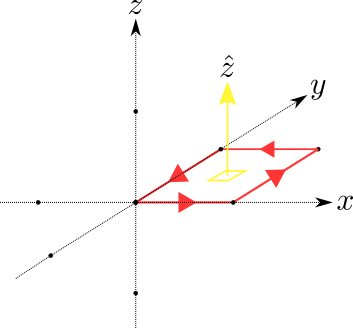
\includegraphics[width=0.4\textwidth]{plaquette.png}
    \caption{Integration path defined as $\boxdot_z$ along a plaquette of the numerical lattice in the $xy$-plane.}
    \label{fig:LM:Field:Fluc:plaquetteSum}
\end{figure}

To impose an external field on a system with a fluctuating field we divide the link-variables into a fluctuating part $A^f_{\v{r},\mu}$ with periodic boundary conditions
and a constant part $A^0_{\v{r},\mu}$ such that $A_{\v{r},\mu} = A^f_{\v{r},\mu} + A^0_{\v{r},\mu}$. The field is then imposed by setting the constant part such that there is a
net field induction through the system, \eg by setting it to one of the gauges in Section~\ref{sec:LM:Field:LandauGauge} and \ref{sec:LM:Field:SymmLandauGauge}.

%\section{Observables in lattice models}


